\let\negmedspace\undefined
\let\negthickspace\undefined
\documentclass[journal]{IEEEtran}
\usepackage[a5paper, margin=10mm, onecolumn]{geometry}
\usepackage{lmodern} % Ensure lmodern is loaded for pdflatex
\usepackage{tfrupee} % Include tfrupee package

\setlength{\headheight}{1cm} % Set the height of the header box
\setlength{\headsep}{0mm}     % Set the distance between the header box and the top of the text

\usepackage{gvv-book}
\usepackage{gvv}
\usepackage{cite}
\usepackage{amsmath,amssymb,amsfonts,amsthm}
\usepackage{algorithmic}
\usepackage{graphicx}
\usepackage{textcomp}
\usepackage{xcolor}
\usepackage{txfonts}
\usepackage{listings}
\usepackage{enumitem}
\usepackage{mathtools}
\usepackage{gensymb}
\usepackage{comment}
\usepackage[breaklinks=true]{hyperref}
\usepackage{tkz-euclide} 
\usepackage{listings}
\usepackage{gvv}                                        
\def\inputGnumericTable{}                                 
\usepackage[latin1]{inputenc}                                
\usepackage{color}                                            
\usepackage{array}                                            
\usepackage{longtable}                                       
\usepackage{calc}                                             
\usepackage{multirow}                                         
\usepackage{hhline}                                           
\usepackage{ifthen}                                           
\usepackage{lscape}
\begin{document}

\bibliographystyle{IEEEtran}
\vspace{3cm}

\title{9.7.7}
\author{EE24BTECH11005 - Arjun Pavanje}
% \maketitle
% \newpage
% \bigskip
{\let\newpage\relax\maketitle}
\textbf{Question:}
Solve the differential equation $\frac{dy}{dx}+\frac{y^2+y+1}{x^2+x+1}=0$, with initial conditions $y\brak{0}=0$

\solution\\
\textbf{Theoretical Solution:}\\
This is a linear differential equation of the first order.
\begin{align}
  \frac{dy}{dx}= -\frac{y^2+y+1}{x^2+x+1}\\
  \frac{dy}{y^2+y+1}=-\frac{dx}{x^2+x+1}
\end{align}
Integrating on both sides,
\begin{align}
  \int \frac{dy}{y^2+y+1}=-\int \frac{dx}{x^2+x+1}
\end{align}
Completing the square,
\begin{align}
  \int \frac{dy}{\brak{y+\frac{1}{2}}^2 + \brak{\frac{\sqrt{3}}{2}}^2}=-\int \frac{dx}{\brak{x+\frac{1}{2}}^2 + \brak{\frac{\sqrt{3}}{2}}^2}
\end{align}
We know that $\int \frac{dx}{x^2+a^2}=\tan^{-1}\brak{\frac{x}{a}}$
\begin{align}
  \tan^{-1}\brak{\frac{2y+1}{\sqrt{3}}}= -\tan^{-1}\brak{\frac{2x+1}{\sqrt{3}}}+c\\
  \tan^{-1}\brak{\frac{2y+1}{\sqrt{3}}}+\tan^{-1}\brak{\frac{2x+1}{\sqrt{3}}}=c
\end{align}
We know $\tan^{-1}x + \tan^{-1}y = \tan^{-1}\brak{\frac{x+y}{1-xy}}$
\begin{align}
  \tan^{-1}\brak{\frac{2x++2y+2}{2-4xy-2x-2y}}=c
\end{align}
On simplifying we get,
\begin{align}
  \brak{x+y+1}=A\brak{1-x-y-2xy}
\end{align}
Where $A$ is a constant. On substituting initial conditions we get,
\begin{align}
  \brak{x+y+1}&=\brak{1-x-y-2xy}\\
  y&=\frac{-x}{1+x}
\end{align}


\textbf{Computational Solution:}\\
By first principle of derivatives,
\begin{align}
    y^{\prime}\brak{t} = \lim_{h\to 0}\frac{y\brak{t+h} - y\brak{t}}{h}\\
    y\brak{t+h} = y\brak{t} + hy^{\prime}\brak{t}
\end{align}
If we repeat the above proccess iteratively, we obtain the points to plot. Taking smaller step-size $h$ will give more accurate plots. On discretizing the proccess we get,

\begin{align}  
  y\brak{x_{n+1}}&=y\brak{x_n} + h y^{\prime}\brak{x_n}\\
  x_{n+1}&=x_n+h
\end{align}
If we denote $y\brak{x_n}$ as $y_n$, the equation $\brak{14}$ becomes,
\begin{align}
  y_{n+1}=y_n+hy^{\prime}_n
\end{align}
The above equation is the general difference equation.\\

In the given question,
\begin{align}
  y^{\prime}=-\frac{y^2+y+1}{x^2+x+1}
\end{align}
Difference Equation can be written as,
\begin{align}
  y_{n+1}=y_n- h \brak{\frac{y_n^2+y_n+1}{x_n^2+x_n+1}
}
\end{align}
Below is a comparission between Simulated Plot and Theoretical Plot.
\begin{figure}[h!]
   \centering
   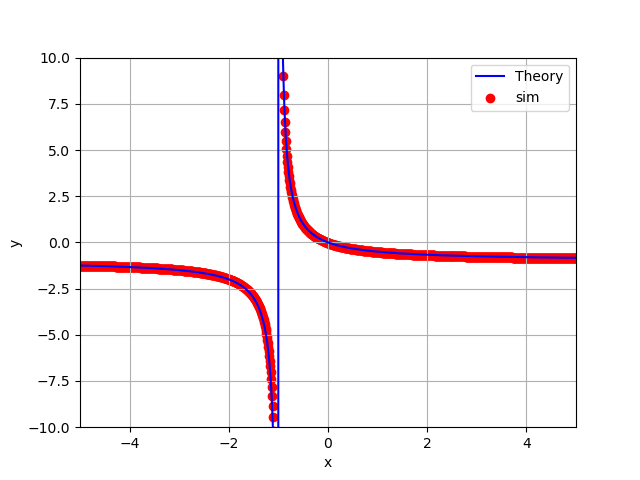
\includegraphics[width=1\columnwidth]{figs/fig.png}
   \caption{Computational vs Theoretical solution of $ \frac{dy}{dx}=-\frac{y^2+y+1}{x^2+x+1}$}
   \label{stemplot}
\end{figure}
\end{document}
